\documentclass{article}
\usepackage[T1]{fontenc}
\usepackage{lmodern}
\usepackage{graphicx}
\usepackage{amsmath,amssymb}
\usepackage[a4paper,margin=2cm]{geometry}
\usepackage[absolute,overlay]{textpos}
\setlength{\TPHorizModule}{1mm}
\setlength{\TPVertModule}{1mm}
\usepackage[indonesian]{babel}
\usepackage{hyperref}
\setlength{\emergencystretch}{2em}
% unit: Halaman 91

\begin{document}

% === Halaman 91 (llm) ===

\vspace{280.37mm}

Perbedaan ChaCha dengan Salsa:

\vspace{76.63mm}

1. Initial state

\vspace{40mm}

2. Quarter round QR

\begin{align*}
a &\leftarrow a + b; \quad d \leftarrow d \oplus a; \quad d \leftarrow d \lll 16; \\
c &\leftarrow c + d; \quad b \leftarrow b \oplus c; \quad b \leftarrow b \lll 12; \\
a &\leftarrow a + b; \quad d \leftarrow d \oplus a; \quad d \leftarrow d \lll 8; \\
c &\leftarrow c + d; \quad b \leftarrow b \oplus c; \quad b \leftarrow b \lll 7;
\end{align*}

% deskripsi: Tabel initial state of ChaCha yang terdiri dari konstanta, key, counter, dan nonce.
% bbox normalisasi: [0.1070, 0.1760, 0.4080, 0.4340]
\begin{textblock*}{63.21mm}(22.47mm,52.27mm)
\noindent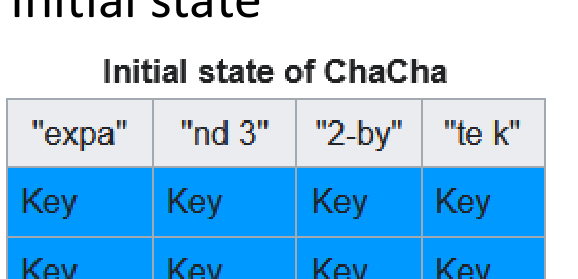
\includegraphics[width=63.21mm,height=76.63mm]{../../images/llm/page_091_img_01.png}%
\end{textblock*}

% deskripsi: Diagram alir operasi Quarter Round (QR) pada ChaCha dengan simbol penjumlahan, XOR, dan rotasi bit.
% bbox normalisasi: [0.5810, 0.0000, 0.9720, 0.9440]
\begin{textblock*}{82.11mm}(122.01mm,0.00mm)
\noindent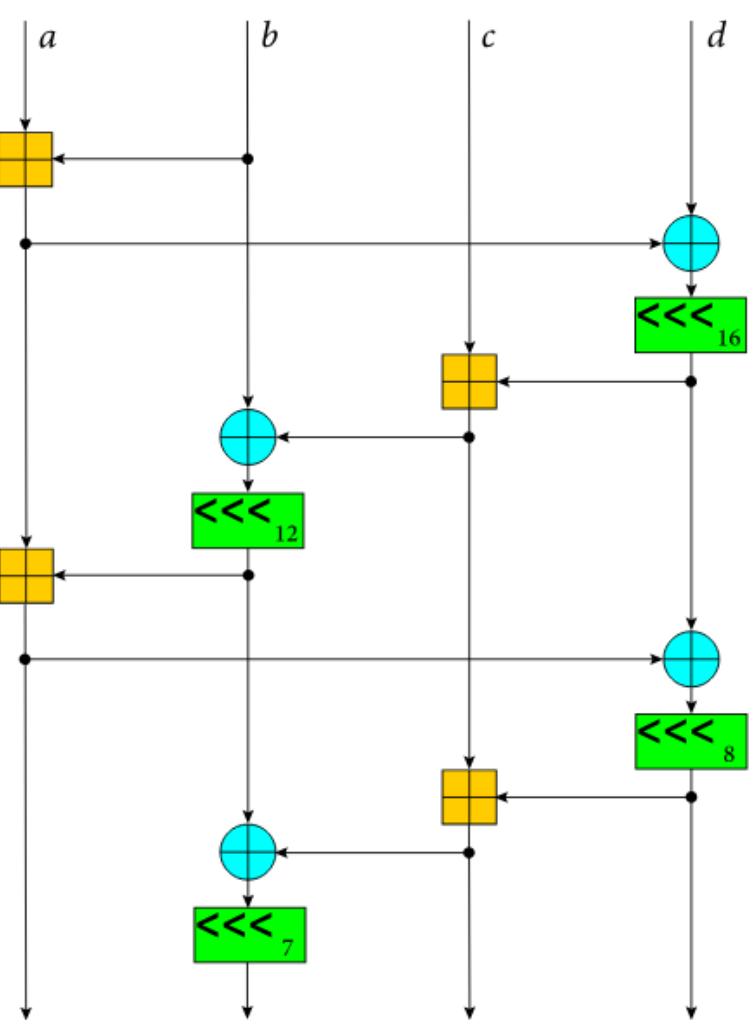
\includegraphics[width=82.11mm,height=280.37mm]{../../images/llm/page_091_img_02.png}%
\end{textblock*}

\end{document}
